\section{Auswertung}
\label{sec:Auswertung}

\subsection{Der Brechungsindex}

Zur Auswertung der aufgenommenen Messwerte werden die Brechungsindizes $n$ bei senkrechter bzw. paralleler Polarisation benötigt.
Diese können aus der Umstellung von \eqref{eq:E_rsenkrecht+snell} und \eqref{eq:E_parSnellius} gewonnen werden.
Dazu sei anzumerken, dass die gemessene Intensität proportional zum Amplitudenquadrat ist.
Es gilt also

\begin{equation}
    \frac{I_r}{I_e} \sim \frac{E_r}{E_e}^2 = E^2 \,.
    \label{eq:Intensprop}
\end{equation}


\subsubsection{Brechungsindex bei senkrechter Polarisation}
\label{subsubsec:senkPol}

Mithilfe der Definition von $E$ in \eqref{eq:Intensprop} wird \eqref{eq:E_rsenkrecht+snell} zu 

\begin{equation*}
    E_\perp = \left| \frac{\left( \sqrt{n^2 - \sin^2(\alpha)} - \cos^2(\alpha) \right)^2}{n^2 - 1} \right| \,.
\end{equation*} \\

Nach $n$ umgestellt ergibt sich dann
\begin{equation}
    n = \sqrt{1 + \frac{4 E \cos^2(\alpha)}{(E-1)^2}} \,.
    \label{eq:nsenkrecht}
\end{equation} \\

In \autoref{tab:Messung1} sind die Messwerte für die senkrechte Polarisation dargestellt. Zusätzlich dazu ist der Intensitätsquotient $E \sim \dfrac{I_r}{I_e}$ sowie 
der nach \eqref{eq:nsenkrecht} berechnete Brechungsindex aufgetragen.

\begin{table}[H]
    \centering
    \caption{Messreihe für senkrechte Polarisation.}
    \label{tab:Messung1}
    \begin{tabular}{S[table-format=2.0] S[table-format=3.0] S[table-format=1.3] S[table-format=1.3]}
      \toprule
        {Winkel $\alpha$ in $\unit{\degree}$} & {Strom $\mathbin{/} \unit{\micro\ampere}$} & {$\sqrt{\frac{\text{Ref}}{\text{Einf}}}$} & {$n$}\\
      \midrule
       5       &        56     &     0.287     &    3.297    \\ 
      10       &        62     &     0.317     &    3.535    \\
      15       &        67     &     0.343     &    3.711    \\
      20       &        69     &     0.353     &    3.714    \\
      25       &        71     &     0.364     &    3.688    \\
      30       &        72     &     0.369     &    3.583    \\
      35       &        77     &     0.394     &    3.635    \\
      40       &        85     &     0.435     &    3.797    \\
      45       &        84     &     0.430     &    3.480    \\
      50       &        96     &     0.492     &    3.745    \\
      55       &       100     &     0.512     &    3.562    \\
      60       &       102     &     0.523     &    3.231    \\
      65       &       108     &     0.553     &    3.020    \\
      70       &       112     &     0.574     &    2.654    \\
      75       &       139     &     0.712     &    3.214    \\
      80       &       157     &     0.805     &    3.355    \\
      85       &       160     &     0.820     &    2.025    \\
      \bottomrule
    \end{tabular}
  \end{table}

  Gemittelt ergibt sich somit ein Brechungsindex von

  \begin{equation*}
      n_\perp = 3,4 \pm 0,4 \,. 
  \end{equation*}

\subsubsection{Brechungsindex bei paralleler Polarisation}

Analog ergibt sich \eqref{eq:E_parSnellius} zu

\begin{equation*}
    E_\parallel = \left| \frac{n^2 \, \cos(\alpha) - \sqrt{n^2 - \sin^2(\alpha)}}{n^2 \, \cos(\alpha) + \sqrt{n^2 - \sin^2(\alpha)}} \right| \,.
\end{equation*} \\

Umgestellt nach $n$ folgt

\begin{equation*}
    n_{1,2} = \sqrt{ \frac{1}{2} \left(  \frac{E_{\text{r}\parallel} + E_{\text{e}\parallel}}{E_{\text{r}\parallel} - E_{\text{e}\parallel}} \frac{1}{\cos{\alpha}}\right)^2         \pm \sqrt { \frac{1}{4} \left(  \frac{E_{\text{r}\parallel} + E_{\text{e}\parallel}}{E_{\text{r}\parallel} - E_{\text{e}\parallel}} \frac{1}{\cos{\alpha}}\right)^4         - \left( \frac{E_{\text{r}\parallel} + E_{\text{e}\parallel}}{E_{\text{r}\parallel} - E_{\text{e}\parallel}} \right)^2 \tan^2{\alpha} }    } \, ,
\end{equation*}

wobei die positive Lösung gewählt wird, da dort physikalisch sinnvolle Lösungen herrauskommen.\\

Wie bereits in \autoref{subsubsec:senkPol} sind in \autoref{tab:Messung2} die Messdaten, das Intensitätsverhältnis sowie der Brechungsindex für parallel polarisiertes Licht aufgetragen.

\begin{table}[H]
    \centering
    \caption{Messreihe für parallele Polarisation.}
    \label{tab:Messung2}
    \begin{tabular}{S[table-format=2.0] S[table-format=2.2] S[table-format=1.3] S[table-format=2.2]}
      \toprule
        {Winkel $\alpha$ in $\unit{\degree}$} & {Strom $\mathbin{/} \unit{\micro\ampere}$} & {$\sqrt{\frac{\text{Ref}}{\text{Einf}}}$} & {$n$}\\
      \midrule
       5       &       62.00    &     0.317    &    3.587  \\
      10       &       62.00    &     0.317    &    3.617  \\
      15       &       60.00    &     0.307    &    3.579  \\
      20       &       58.00    &     0.297    &    3.571  \\
      25       &       55.00    &     0.282    &    3.547  \\
      30       &       50.00    &     0.256    &    3.459  \\
      35       &       50.00    &     0.256    &    3.659  \\
      40       &       46.00    &     0.235    &    3.702  \\
      45       &       39.00    &     0.200    &    3.631  \\
      50       &       34.00    &     0.174    &    3.718  \\
      55       &       24.00    &     0.123    &    3.559  \\
      60       &       18.00    &     0.092    &    3.685  \\           
      62       &       15.00    &     0.076    &    3.707  \\
      66       &        8.80    &     0.045    &    3.734  \\
      70       &        3.20    &     0.016    &    3.739  \\
      72       &        1.40    &     0.007    &    3.795  \\
      74       &        0.85    &     0.004    &    4.108  \\
      75       &        0.85    &     0.004    &    4.381  \\
      78       &        5.10    &     0.026    &    6.650  \\
      80       &       11.00    &     0.056    &    9.337  \\  
      81       &       17.00    &     0.087    &    11.742  \\
      82       &       25.00    &     0.128    &    15.196  \\
      83       &       35.00    &     0.179    &    20.266  \\
      84       &       50.00    &     0.256    &    29.192  \\   
      85       &       52.00    &     0.266    &    35.976  \\
      \bottomrule
    \end{tabular}
\end{table}

Gemittelt ergibt sich hier ein Wert von
\begin{equation*}
    n = 3,71 \pm 0,21
\end{equation*}
für den Brechungsindex.

\newpage

\subsubsection{Bestimmung des Brechungsindexes mithilfe des Brewsterwinkels}

Wie in \autoref{tab:Messung2} zu erkennen, liegt bei einem Winkel zwischen $74°$ und $75°$ ein Stromminimum vor.

Der Brewsterwinkel liegt also näherungsweise bei
\begin{equation*}
    \alpha_p = 74,5 ° \,.
\end{equation*}

Aus
\begin{equation*}
    \tan(\alpha) = n 
\end{equation*}
ergibt sich

\begin{equation*}
    n_{\alpha_p} = 3,606 \,.
\end{equation*}

In \autoref{fig:graph1} sind nun abschließend die Mess- und Theoriewerte grafisch aufgetragen. Die Theoriekurven nutzen dabei den berechneten durchschinttlichen Brechungsindex

\begin{equation*}
    \bar{n} = 3,57 \pm 0,16 \,.
\end{equation*}

\begin{figure}
    \centering
    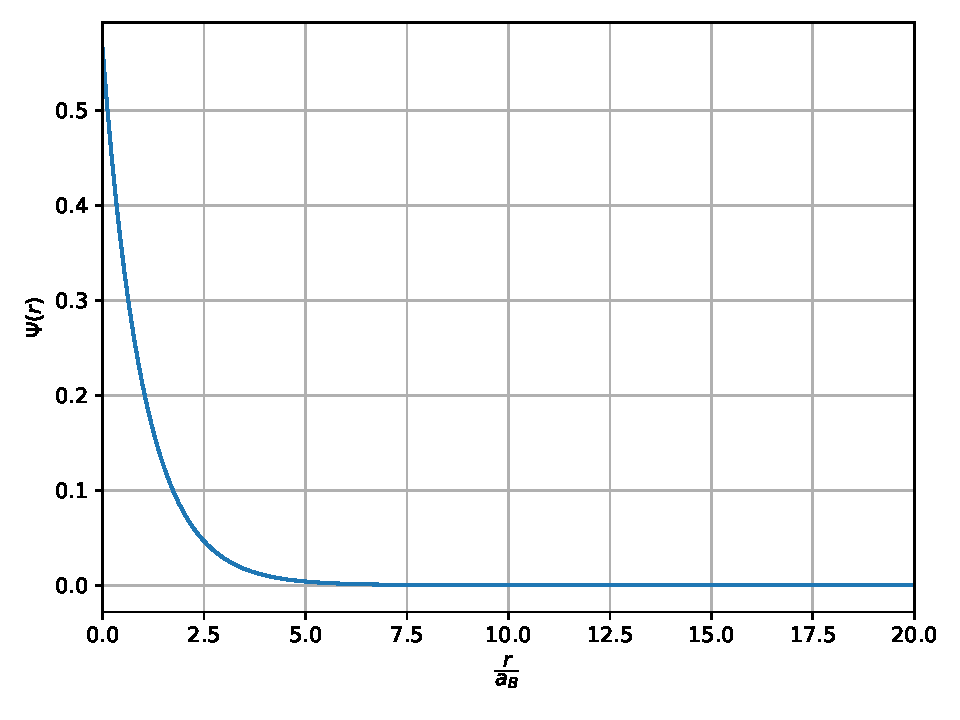
\includegraphics{build/Graph_a.pdf}
    \caption{Intensitätsverhältnis in Abhängigkeit vom Winkel $\alpha$.}
    \label{fig:graph1}
\end{figure}
